\section{Comparisons with HPWL and QCLIQUE} \label{sec:comparisons_with_hpwl_and_qclique}

In the last section of this chapter, the parameters that were chosen in the previous sections are used
to compare the minimization of the \(\NLSE\)/\(\NWA\) netlength estimations
with the results of minimizing \(\HPWL\) or \(\QCLIQUE\).
The parameters that were chosen are:
\begin{itemize}
 \item Objective function: \(T_{\NWA_\gamma}\) with \(\gamma = 10^5\)
 \item Start vector: CENTER
 \item Optimization method: Nesterov's accelerated gradient method
 \item The step size strategy: \texttt{barzilai-borwein}
 \item The stopping criterion: After 200 iterations
\end{itemize}

There are three main categories for this comparison, namely solution quality,
weighted total HPWL and runtime.
We will first investigate the latter two in \cref{table:hpwl_qclique_netlength_comparisons,table:hpwl_qclique_runtime_comparisons}.
In both tables, the columns specify which objective function was minimized while the rows show the results for different chips.
For \cref{table:hpwl_qclique_netlength_comparisons} the columns are subdivided to show the weighted wirelength based on HPWL and NWA
of the final placement.

\begin{table}[ht] 
 \centering
 \begin{tabular}{c c c c c c c c}
  Instance       & \multicolumn{2}{c}{\(\min\) NWA} & \multicolumn{2}{c}{\(\min\) QCLIQUE} & \multicolumn{2}{c}{\(\min\) HPWL} \\
                 & NWA            & HPWL              & NWA            & HPWL                  & NWA            & HPWL               \\
  \hline
  \texttt{Chip1} & 3.741          & 5.019             & 3.723          & 8.690                 & 3.643          & 4.020              \\
  \texttt{Chip2} & 3.190          & 4.353             & 3.431          & 8.166                 & 3.330          & 3.691              \\
  \texttt{Chip3} & 3.971          & 5.820             & 4.739          & 8.577                 & 3.552          & 3.748              \\
  \texttt{Chip4} & 0.192          & 1.228             & 0.188          & 1.369                 & 0.466          & 0.594              \\
 \end{tabular}
 \caption{The weighted wirelengths after minimizing different objective functions in meters}
 \label{table:hpwl_qclique_netlength_comparisons}
\end{table}

\begin{table}[ht] 
 \centering
 \begin{tabular}{c c c c c c c c}
  Instance       & \# Pins   & \(\min\) NWA & \(\min\) QCLIQUE & \(\min\) HPWL \\
  \hline
  \texttt{Chip1} & 5,600,000 & 887.025        & 42.599             & 17325.760       \\
  \texttt{Chip2} & 5,400,000 & 755.941        & 42.811             & 17258.766       \\
  \texttt{Chip3} & 2,200,000 & 311.384        & 13.402             & 6248.931        \\
  \texttt{Chip4} & 800,000   & 155.498        & 2.433              & 1588.552        \\
 \end{tabular}
 \caption{The runtimes of minimizing different objective functions in seconds}
 \label{table:hpwl_qclique_runtime_comparisons}
\end{table}

Regarding the weighted HPWL, minimizing NWA produces lower values than minimizing QCLIQUE
but the decrease is about 45\% for \texttt{Chip1} and \texttt{Chip2} and roughly 10\% for \texttt{Chip4}.
The closer the cells are to the center the higher the HPWL decrease so this might be caused by starting at the center
and not by NWA being a better approximation of HPWL than QCLIQUE.
Also note that for \texttt{Chip1} and \texttt{Chip3} the NWA wirelength is lower after minimizing QCLIQUE than after minimizing NWA.
This certainly underlines one of the earlier observations that very different placements can lead to similarly low values
of NWA but it could also indicate that this is not the right minimization technique if it performs worse
than a different technique with a completely different objective function.
One interesting option would be to minimize QCLIQUE with the CG method first
as NLSE/NWA seem to be rather similar to QCLIQUE for high \(\gamma\)-values (also see \cref{fig:objective_convergence_by_start_vectors})
and then optimize the result futher with NLSE/NWA and smaller \(\gamma\) values.

When comparing runtimes, it is clear that minimizing QCLIQUE is much faster than NWA.
Only about 3 to 11 NAG iterations are possible in the timespan needed for QCLIQUE to converge.
Especially on the larger chips, 11 iterations are almost nothing.
Minimizing HPWL optimally on the other hand is much slower than using NWA.

Let us now get to the placement plots that are produced by minimizing these objective functions:
\Cref{fig:placement_Chip1_depending_on_objective_function,fig:placement_Chip2_depending_on_objective_function,fig:placement_Chip3_depending_on_objective_function,fig:placement_Chip4_depending_on_objective_function}
show the placement plots after minimizing each objective function.
In almost all of these cases the QCLIQUE results are much better at spreading out the cells
and therefore more useful for a subsequent partitioning step than the placements produced by minimizing NWA.
The only exception is \texttt{Chip4} on which both netlength estimations produce very similar results
but using NWA has a runtime that is 70x higher.

All in all this is rather disappointing.
\Cref{sec:baseline} showed that in general the NLSE and NWA netlength estimations are able to produce
somewhat useful placements for a partitioning step but they need an extreme amount of resources to do so.
Once the number of iterations is restricted to bring down the runtime the results cannot compete with QCLIQUE anymore.

\begin{figure}[p]
 \centering

 \begin{subfigure}{.6\textwidth}
  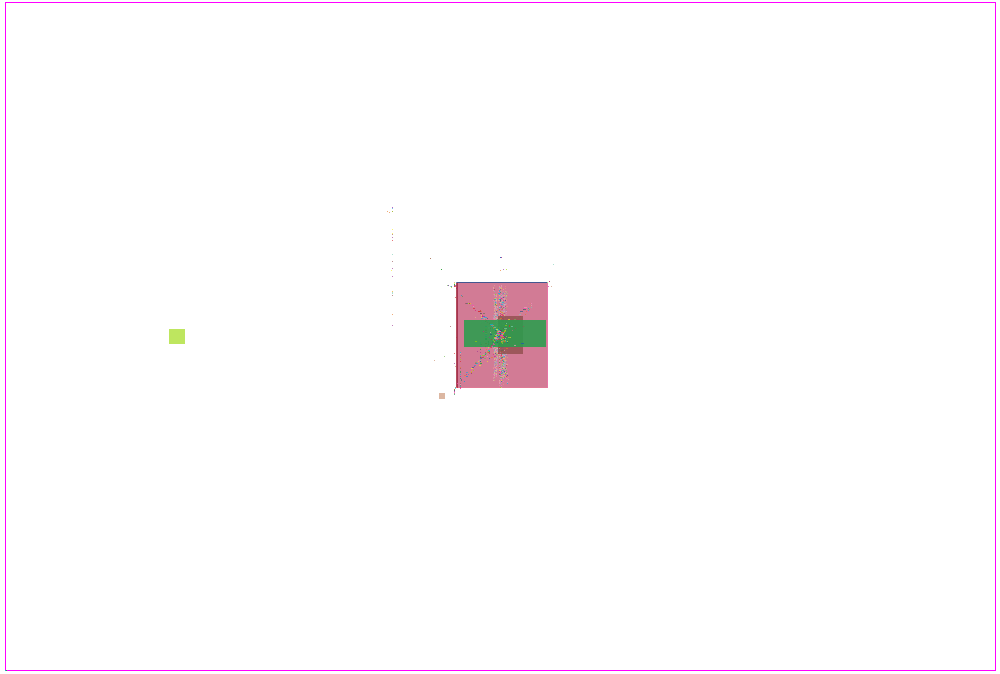
\includegraphics[width=\textwidth]{hpwl_qclique_comparisons/placement_Chip1_NWA.png}
  \caption{NWA}
 \end{subfigure}
 
 \bigskip
 
 \begin{subfigure}{.6\textwidth}
  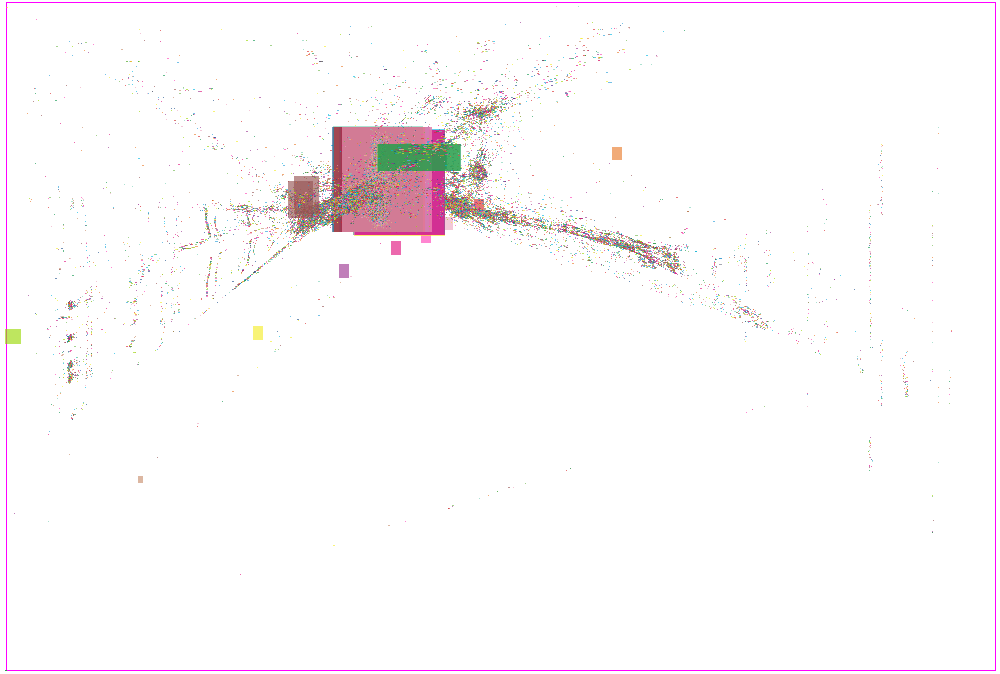
\includegraphics[width=\textwidth]{hpwl_qclique_comparisons/placement_Chip1_QCLIQUE.png}
  \caption{QCLIQUE}
 \end{subfigure}
 
 \bigskip
 
 \begin{subfigure}{.6\textwidth}
  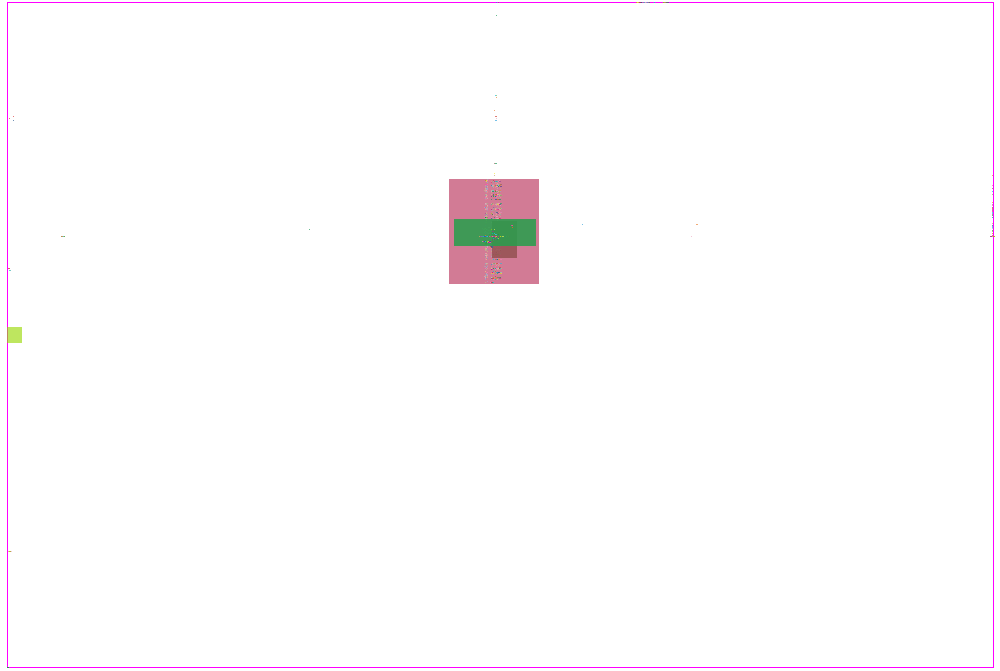
\includegraphics[width=\textwidth]{hpwl_qclique_comparisons/placement_Chip1_HPWL.png}
  \caption{HPWL}
 \end{subfigure}

 \caption{Placement plots for \texttt{Chip1}}
 \label{fig:placement_Chip1_depending_on_objective_function}
\end{figure}

\begin{figure}[p]
 \centering

 \begin{subfigure}{.6\textwidth}
  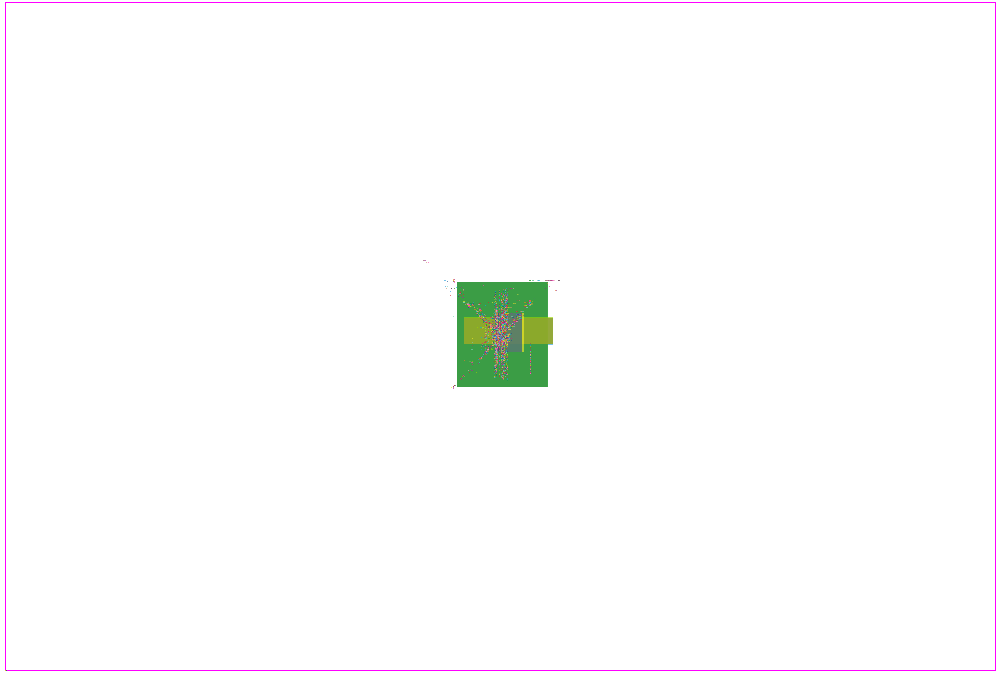
\includegraphics[width=\textwidth]{hpwl_qclique_comparisons/placement_Chip2_NWA.png}
  \caption{NWA}
 \end{subfigure}
 
 \bigskip
 
 \begin{subfigure}{.6\textwidth}
  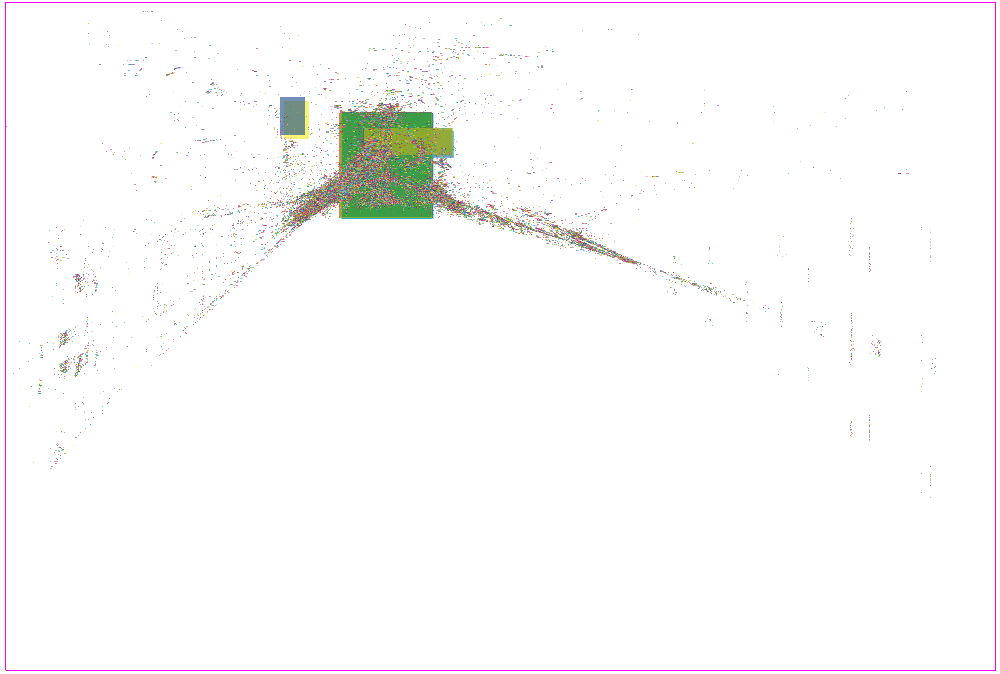
\includegraphics[width=\textwidth]{hpwl_qclique_comparisons/placement_Chip2_QCLIQUE.png}
  \caption{QCLIQUE}
 \end{subfigure}
 
 \bigskip
 
 \begin{subfigure}{.6\textwidth}
  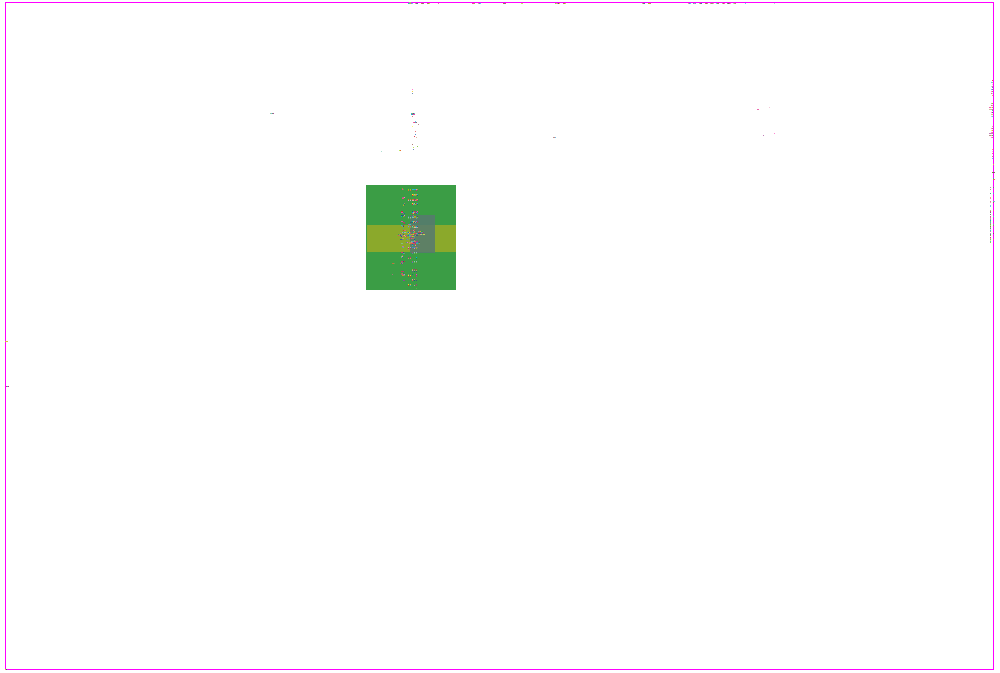
\includegraphics[width=\textwidth]{hpwl_qclique_comparisons/placement_Chip2_HPWL.png}
  \caption{HPWL}
 \end{subfigure}

 \caption{Placement plots for \texttt{Chip2}}
 \label{fig:placement_Chip2_depending_on_objective_function}
\end{figure}

\begin{figure}[p]
 \centering

 \begin{subfigure}{\textwidth}
  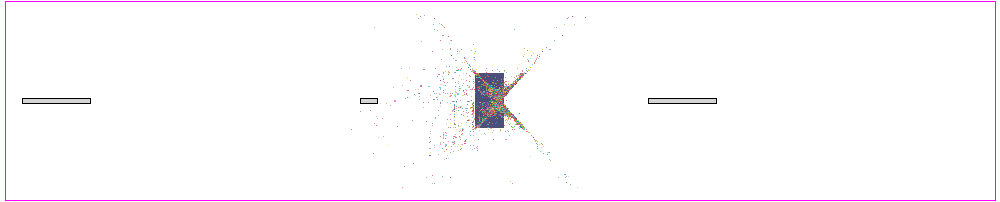
\includegraphics[width=\textwidth]{hpwl_qclique_comparisons/placement_Chip3_NWA.png}
  \caption{NWA}
 \end{subfigure}
 
 \bigskip
 
 \begin{subfigure}{\textwidth}
  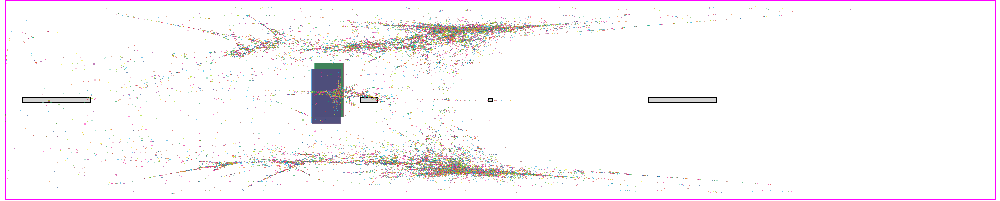
\includegraphics[width=\textwidth]{hpwl_qclique_comparisons/placement_Chip3_QCLIQUE.png}
  \caption{QCLIQUE}
 \end{subfigure}
 
 \bigskip
 
 \begin{subfigure}{\textwidth}
  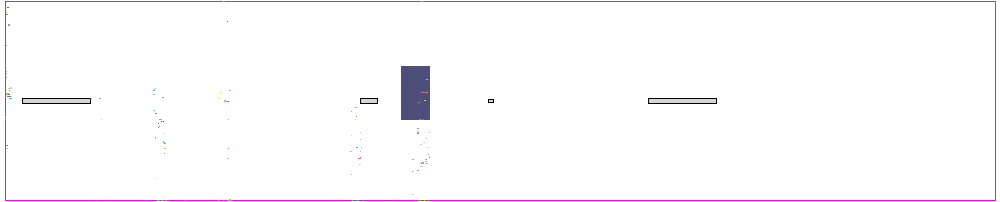
\includegraphics[width=\textwidth]{hpwl_qclique_comparisons/placement_Chip3_HPWL.png}
  \caption{HPWL}
 \end{subfigure}

 \caption{Placement plots for \texttt{Chip3}}
 \label{fig:placement_Chip3_depending_on_objective_function}
\end{figure}

\begin{figure}[p]
 \centering

 \begin{subfigure}{.75\textwidth}
  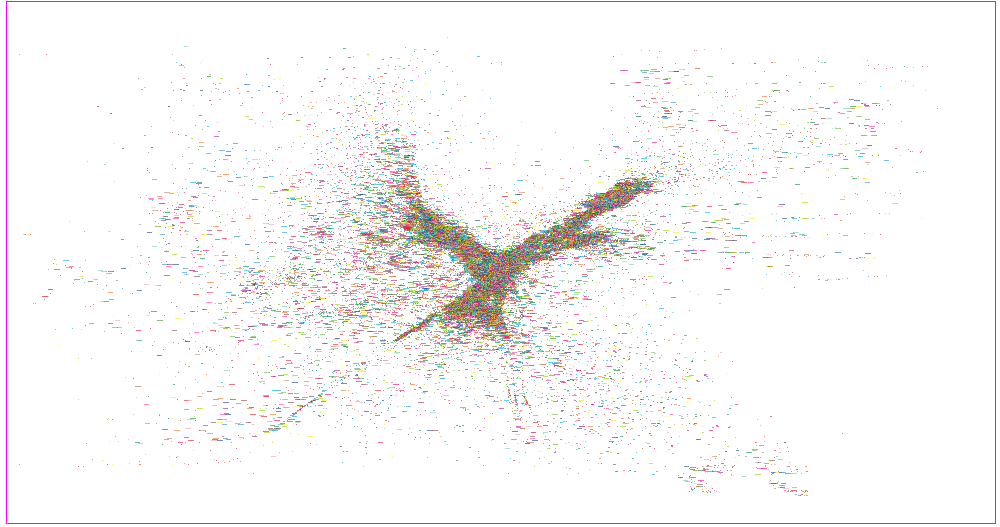
\includegraphics[width=\textwidth]{hpwl_qclique_comparisons/placement_Chip4_NWA.png}
  \caption{NWA}
 \end{subfigure}
 
 \bigskip
 
 \begin{subfigure}{.75\textwidth}
  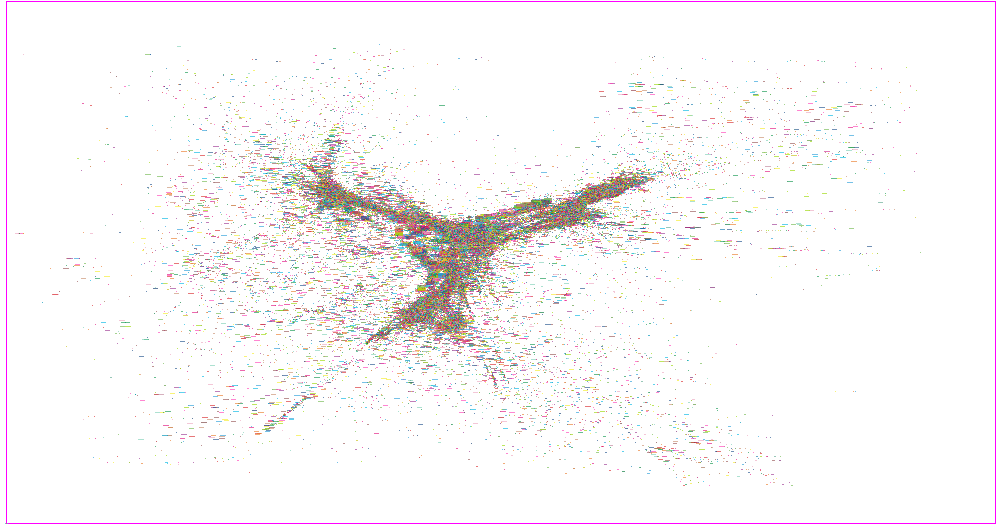
\includegraphics[width=\textwidth]{hpwl_qclique_comparisons/placement_Chip4_QCLIQUE.png}
  \caption{QCLIQUE}
 \end{subfigure}
 
 \bigskip
 
 \begin{subfigure}{.75\textwidth}
  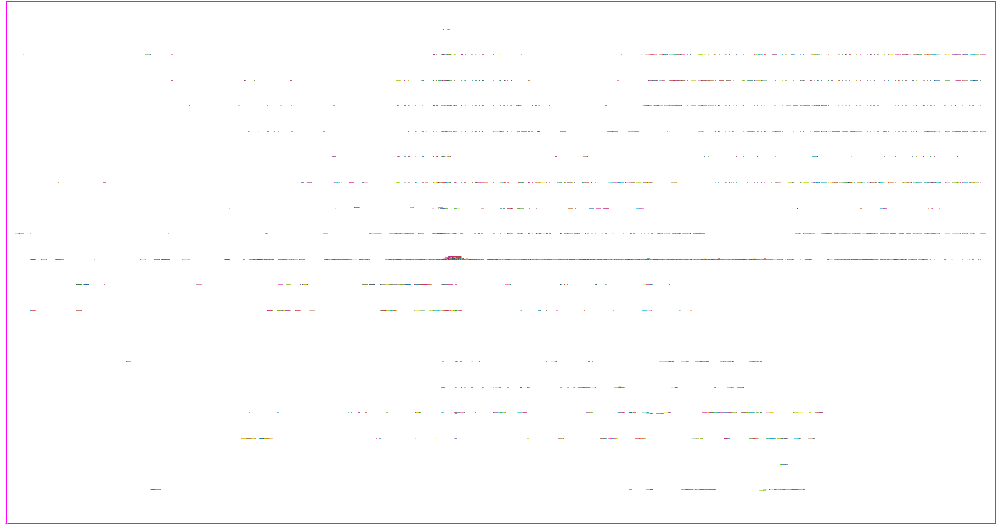
\includegraphics[width=\textwidth]{hpwl_qclique_comparisons/placement_Chip4_HPWL.png}
  \caption{HPWL}
 \end{subfigure}

 \caption{Placement plots for \texttt{Chip4}}
 \label{fig:placement_Chip4_depending_on_objective_function}
\end{figure}
